\section{无限面光源}\label{sec:无限面光源}

\begin{figure}[htbp]
    \centering
    \subfloat[面光源和定向光源]{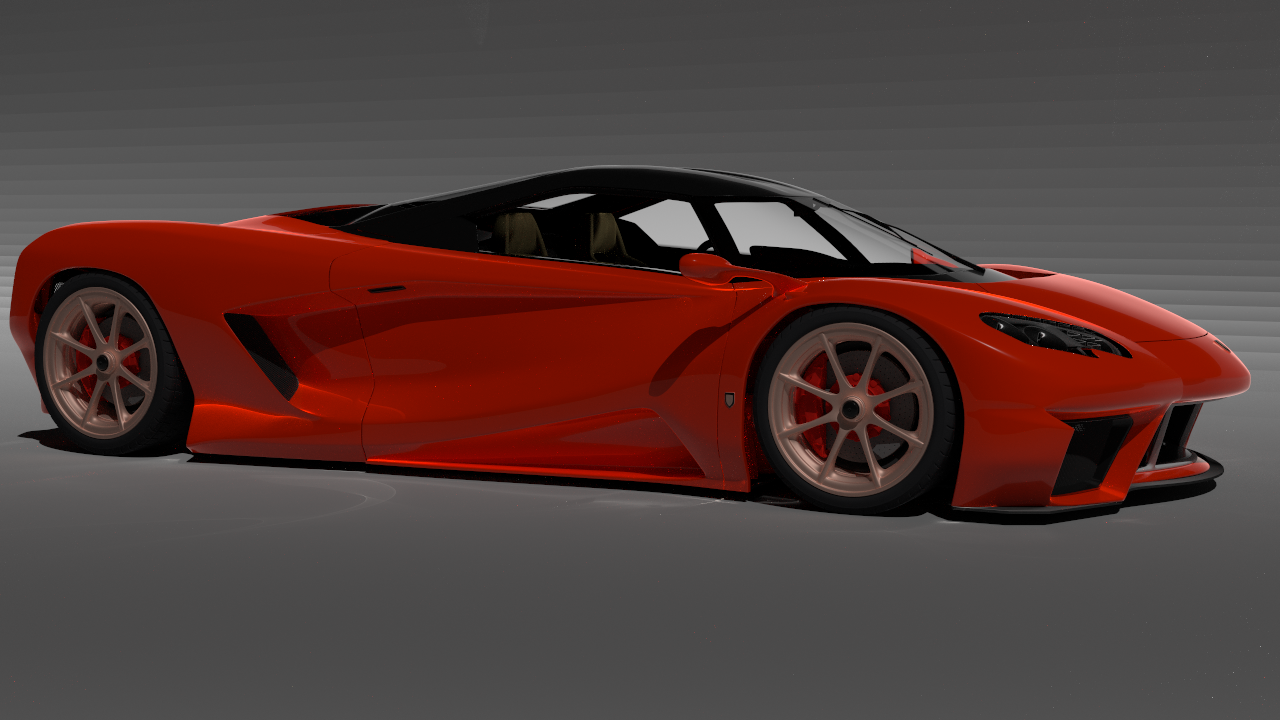
\includegraphics[width=0.5\linewidth]{chap12/car-area-directional.png}\label{fig:12.19.1}}\\
    \subfloat[上午天光]{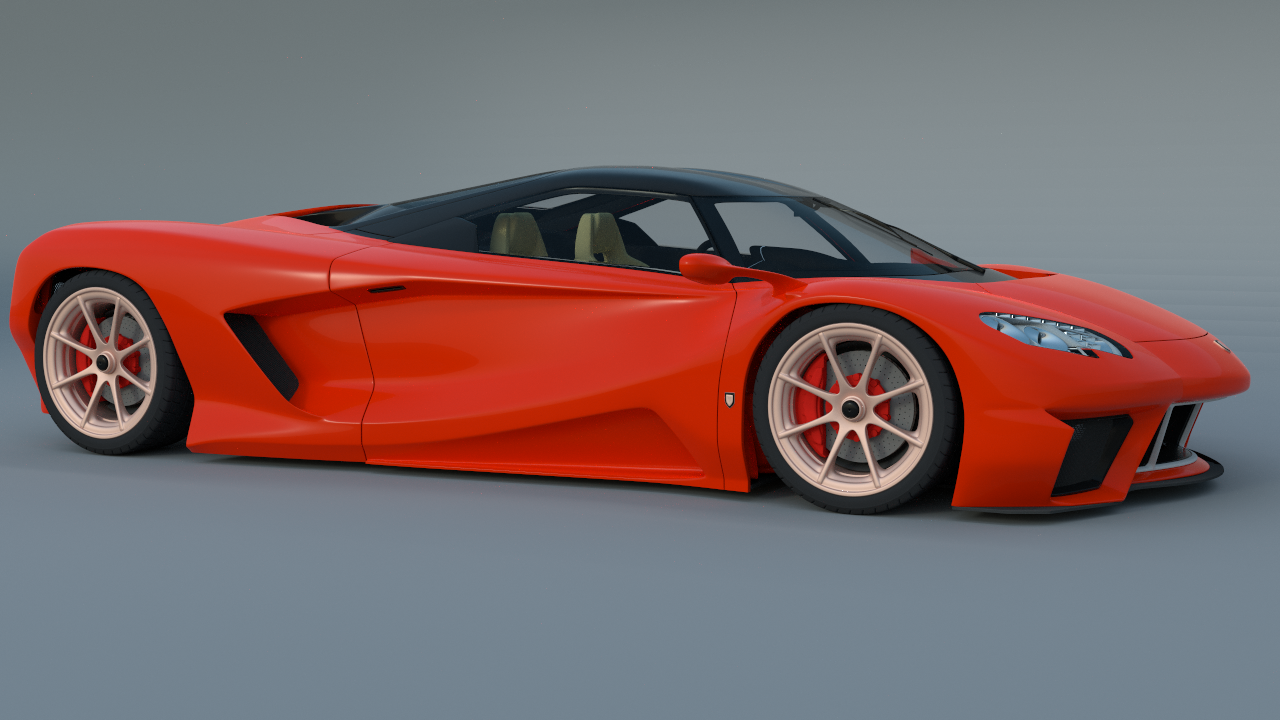
\includegraphics[width=0.5\linewidth]{chap12/car-skylight.png}\label{fig:12.19.2}}\\
    \subfloat[中午天光]{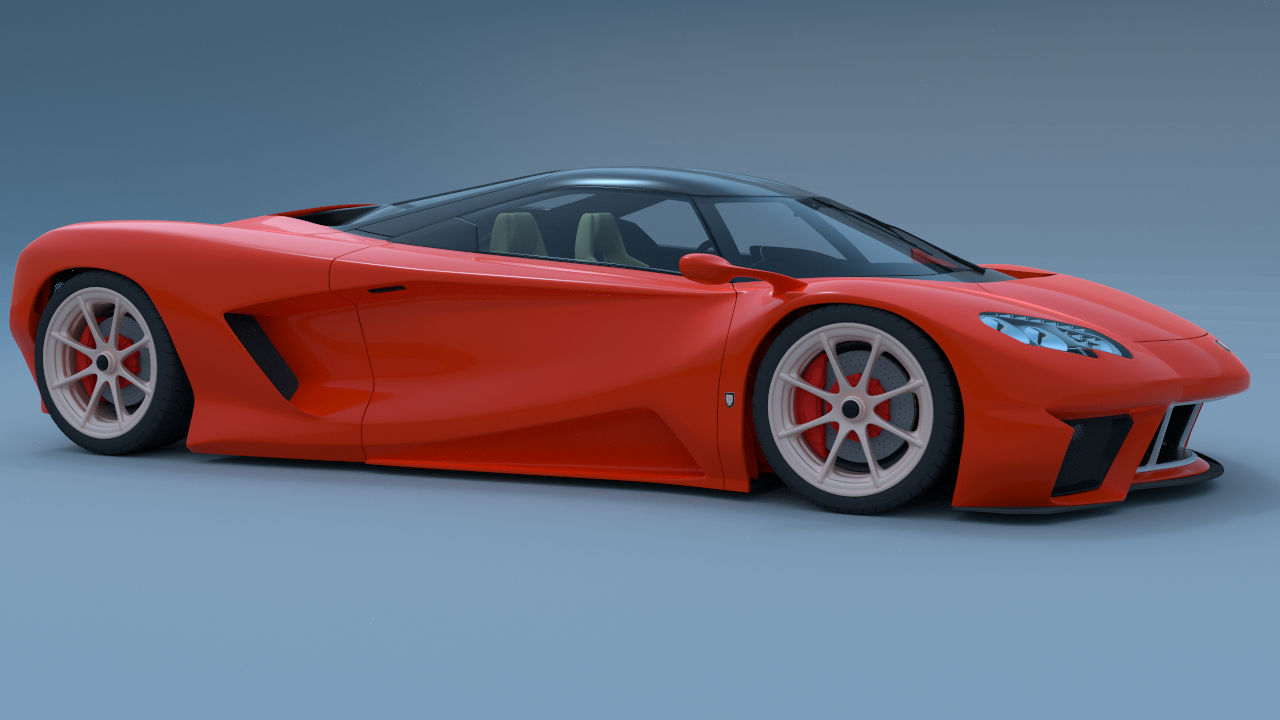
\includegraphics[width=0.5\linewidth]{chap12/car-midday.png}\label{fig:12.19.3}}\\
    \subfloat[傍晚]{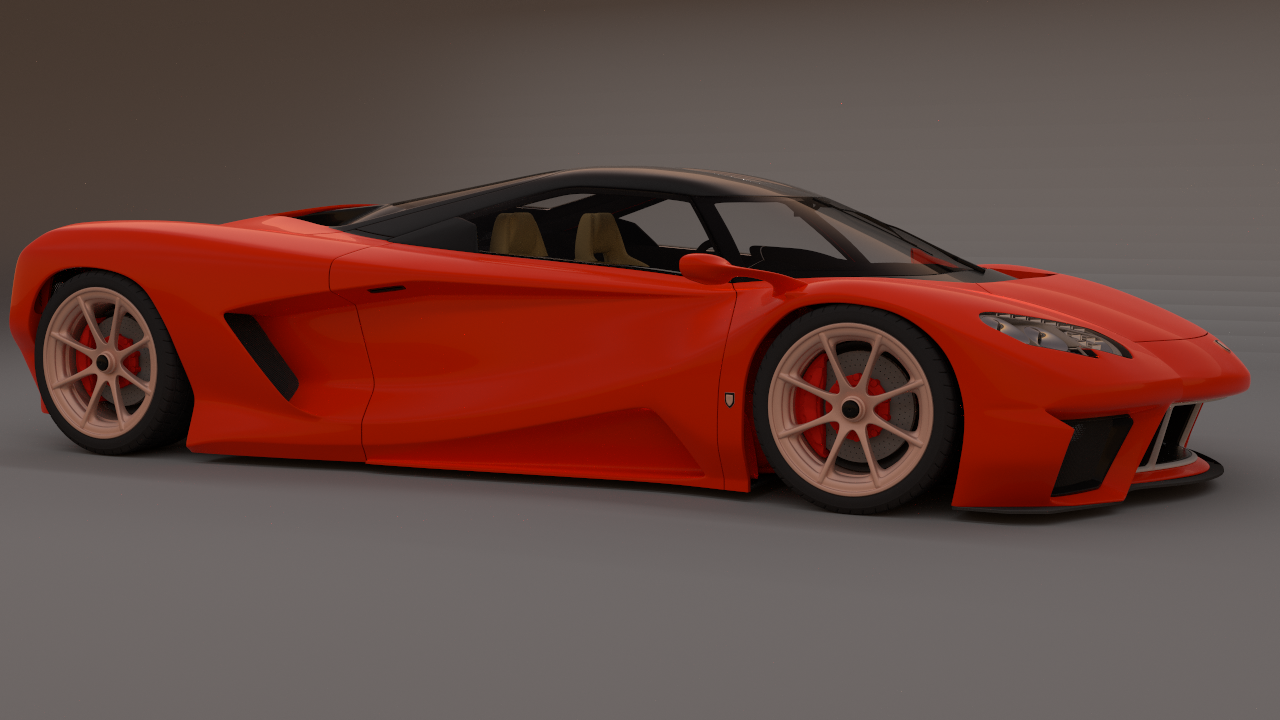
\includegraphics[width=0.5\linewidth]{chap12/car-sunset.png}\label{fig:12.19.4}}\\
    \caption{用(a)面光源和定向光源、(b)来自环境贴图的上午天光、(c)中午天光分布
    以及(d)傍晚环境贴图照明的汽车模型。使用逼真照明分布可以得到更具视觉信服力的图像。
    特别地,伴随来自所有方向的照明时,车漆的光泽反射性质在视觉上明显得多(感谢Yasutoshi Mori提供的模型)。}
    \label{fig:12.19}
\end{figure}

\begin{lstlisting}
`\initcode{InfiniteAreaLight Declarations}{=}`
class `\initvar{InfiniteAreaLight}{}` : public `\refvar{Light}{}` {
public:
    `\refcode{InfiniteAreaLight Public Methods}{}`
private:
    `\refcode{InfiniteAreaLight Private Data}{}`
};
\end{lstlisting}
\begin{lstlisting}
`\refcode{Light Method Definitions}{+=}\lastcode{LightMethodDefinitions}`
`\refvar{Spectrum}{}` `\initvar{Light::Le}{}`(const `\refvar{RayDifferential}{}` &ray) const {
    return `\refvar{Spectrum}{}`(0.f);
}
\end{lstlisting}